\documentclass{article}
\usepackage[a4paper, margin=1.5cm]{geometry}
\title{Stylebot Experiment}
\author{Wafa Johal}

\usepackage{Sweave}
\begin{document}
\Sconcordance{concordance:Results.tex:Results.Rnw:%
1 5 1 1 0 2 1 1 9 1 92 3 1 1 4 39 0 1 2 3 1 2 2 1 1 2 2 1 1 2 2 2 1 2 2 %
1 1 2 2 1 1 1 17 2 1 2 2 1 1 4 2 2 1 1 3 1 2 1 3 1 2 1 3 1 2 1 3 1 2 1 %
3 1 2 1 1 1 17 1 1 1 5 1 2 2 1 2 2 2 1 2 2 2 1 1 3 1 2 1 3 1 2 1 3 1 2 %
1 3 1 2 1 3 1 2 8 1}

\maketitle




\section{Interviews}
% Table created by stargazer v.5.2 by Marek Hlavac, Harvard University. E-mail: hlavac at fas.harvard.edu
% Date and time: jeu, sep 22, 2016 - 13:56:10
\begin{table}[!htbp] \centering 
  \caption{Summary statistics of activities metadata} 
  \label{} 
\begin{tabular}{@{\extracolsep{5pt}}lccccc} 
\\[-1.8ex]\hline 
\hline \\[-1.8ex] 
Statistic & \multicolumn{1}{c}{N} & \multicolumn{1}{c}{Mean} & \multicolumn{1}{c}{St. Dev.} & \multicolumn{1}{c}{Min} & \multicolumn{1}{c}{Max} \\ 
\hline \\[-1.8ex] 
ordre & 16 & 8.500 & 4.761 & 1 & 16 \\ 
age & 16 & 8.688 & 1.014 & 7 & 11 \\ 
p\_robot & 16 & 3.125 & 1.258 & 1 & 5 \\ 
p\_videogame & 16 & 3.500 & 1.414 & 1 & 5 \\ 
p\_bike & 16 & 2.375 & 1.310 & 1 & 5 \\ 
p\_book & 16 & 2.312 & 1.138 & 1 & 4 \\ 
p\_clothes & 16 & 3.688 & 1.537 & 1 & 5 \\ 
p\_homeworks & 16 & 3.375 & 1.147 & 1 & 4 \\ 
p\_play & 16 & 3.562 & 0.892 & 1 & 4 \\ 
p\_teach & 16 & 3.938 & 0.250 & 3 & 4 \\ 
p\_phone & 15 & 1.867 & 1.302 & 1 & 4 \\ 
p\_webbrowser & 15 & 2.067 & 1.335 & 1 & 4 \\ 
prefered\_session & 14 & 1.643 & 0.497 & 1 & 2 \\ 
e\_robot & 13 & 1.077 & 0.277 & 1 & 2 \\ 
e\_videogame & 13 & 2.615 & 1.193 & 1 & 5 \\ 
e\_bike & 12 & 3.250 & 0.965 & 2 & 5 \\ 
e\_book & 12 & 3.417 & 1.379 & 1 & 5 \\ 
e\_clothes & 13 & 4.308 & 0.751 & 3 & 5 \\ 
e\_homeworks & 13 & 3.115 & 0.650 & 2.000 & 4.000 \\ 
e\_play & 13 & 3.115 & 0.618 & 2.000 & 4.000 \\ 
e\_rules & 12 & 3.167 & 0.577 & 2 & 4 \\ 
e\_learn & 13 & 3.500 & 0.577 & 2.500 & 4.000 \\ 
e\_sport & 12 & 3.000 & 0.603 & 2 & 4 \\ 
e\_teach & 12 & 3.500 & 0.674 & 2 & 4 \\ 
e\_outside & 12 & 2.917 & 0.900 & 1 & 4 \\ 
e\_mood & 12 & 3.375 & 0.569 & 2.500 & 4.000 \\ 
e\_phone & 13 & 2.308 & 1.109 & 1 & 4 \\ 
e\_webbrowser & 13 & 2.500 & 0.957 & 1.000 & 4.000 \\ 
\hline \\[-1.8ex] 
\end{tabular} 
\end{table} 
\subsection{General}

\subsubsection{Gender}
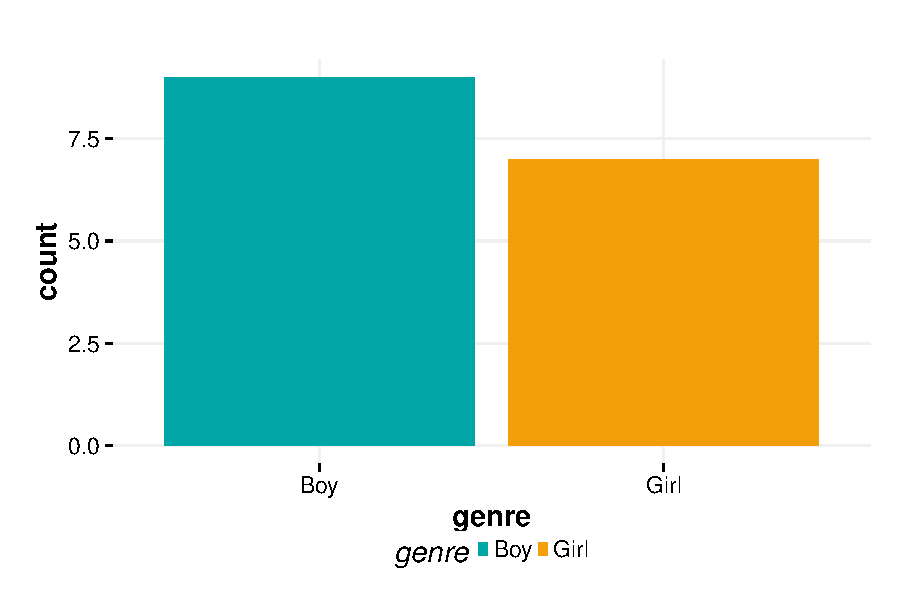
\includegraphics{interviews-plot_gender}

\subsubsection{Age}
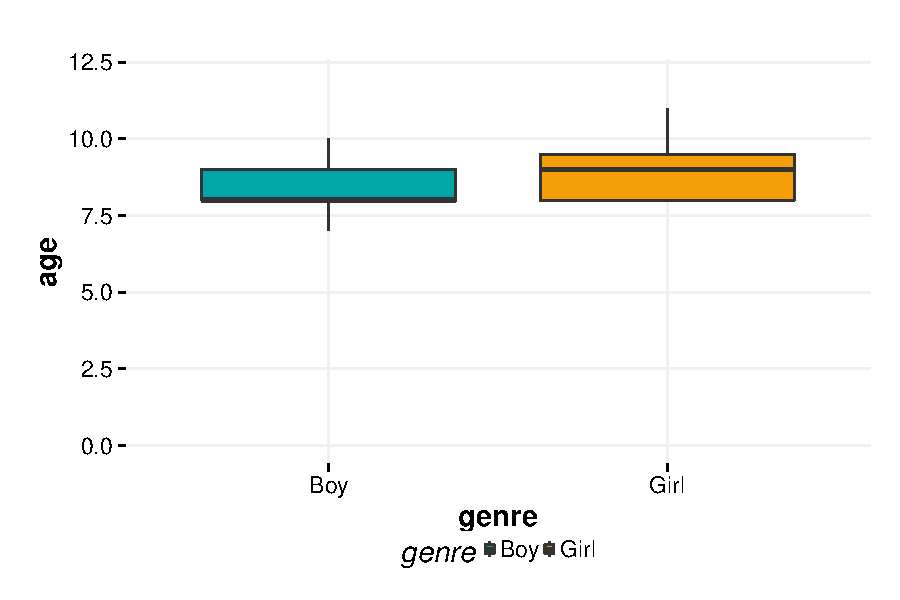
\includegraphics{interviews-plot_gender_age}

\subsubsection{order}
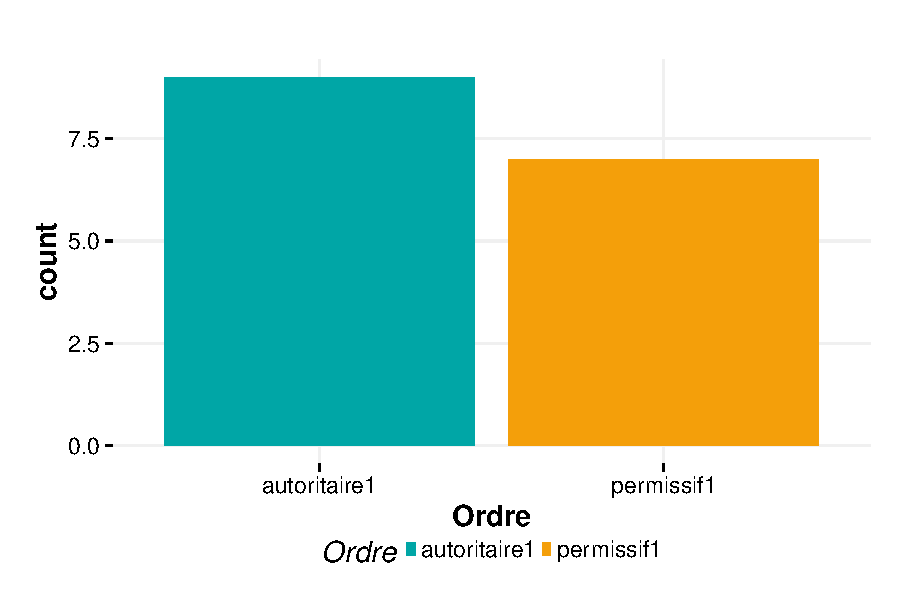
\includegraphics{interviews-plot_order}


\subsubsection{Preferred style parent}
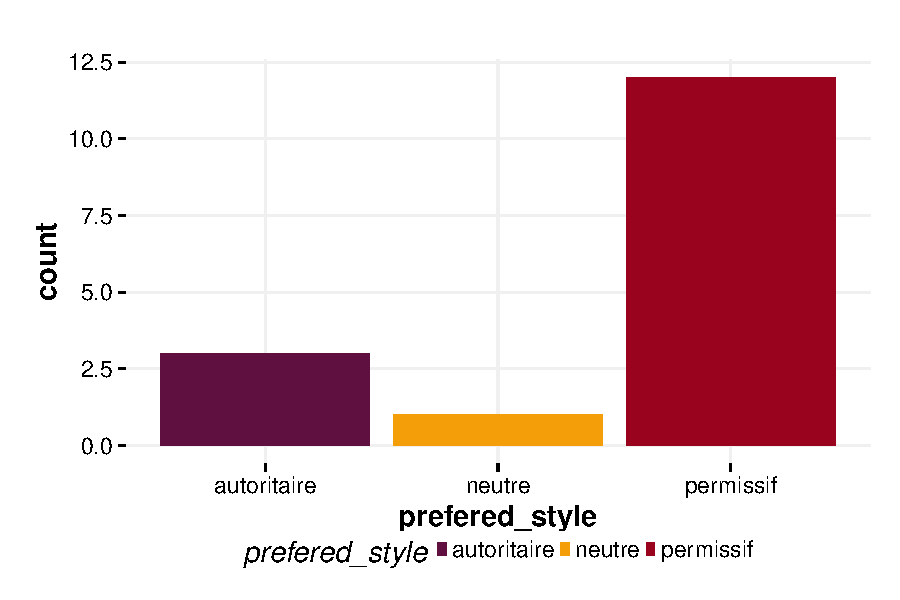
\includegraphics{interviews-plot_preferred_style_parent}

\subsubsection{Preferred style children}
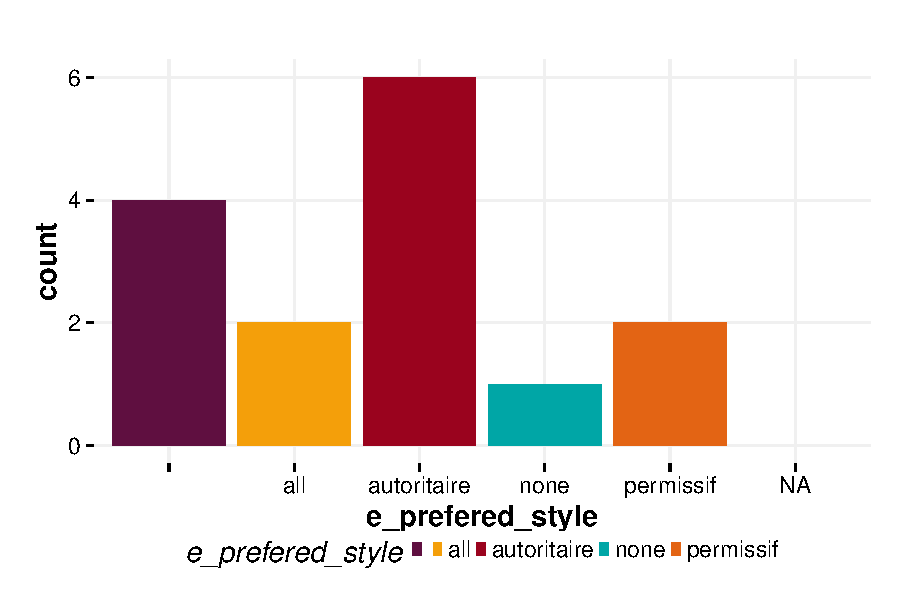
\includegraphics{interviews-plot_preferred_style_child}

\subsection{COIRS - CHILD ORIENTAION IN INTERACTING WITH ROBOT}

The following plot shows the average ranking for children for each of the object (1: first in the child's wish list)

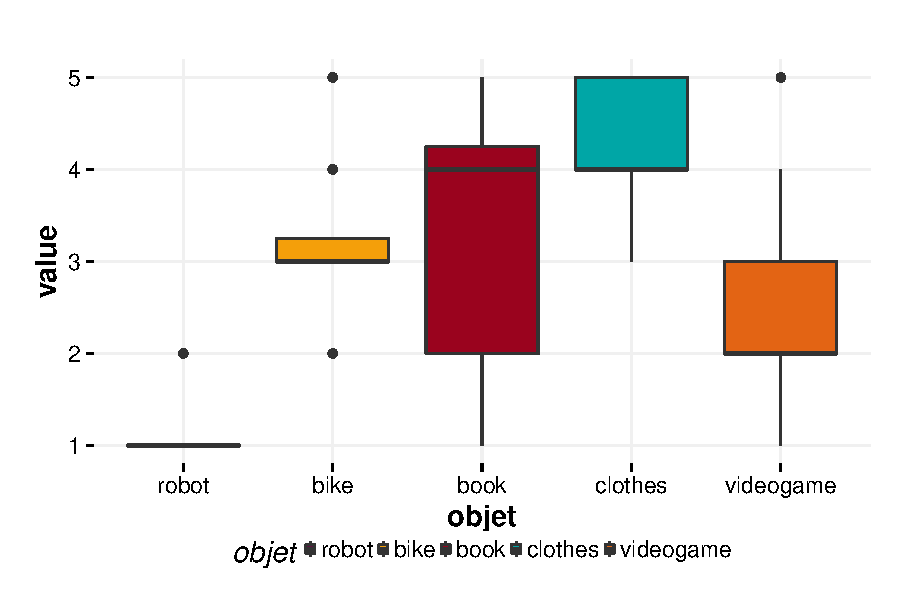
\includegraphics{interviews-plot_coirs_child}

The following plot shows the average ranking for parents for each of the object (1: first in the parent's wish list as a gift for thei child)
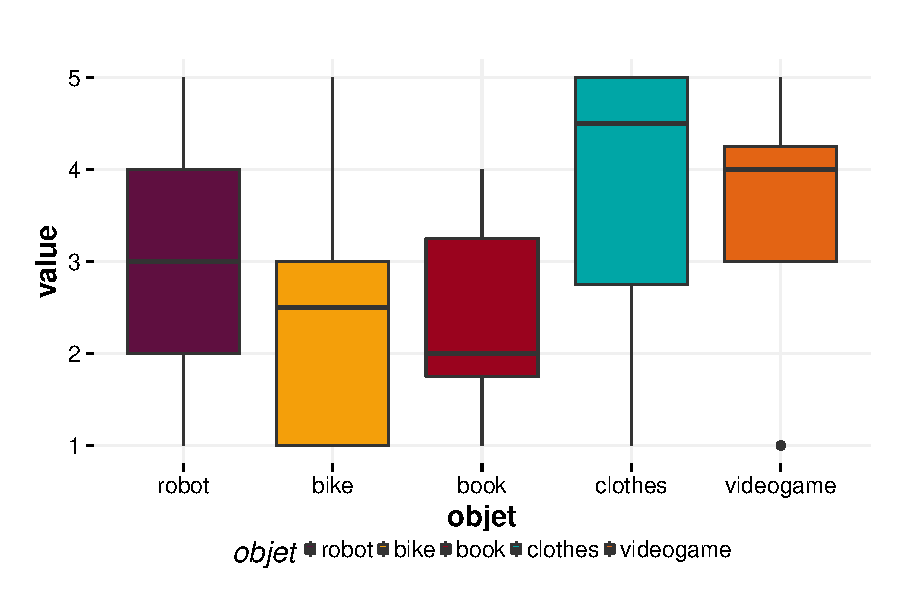
\includegraphics{interviews-plot_coirs_parent}

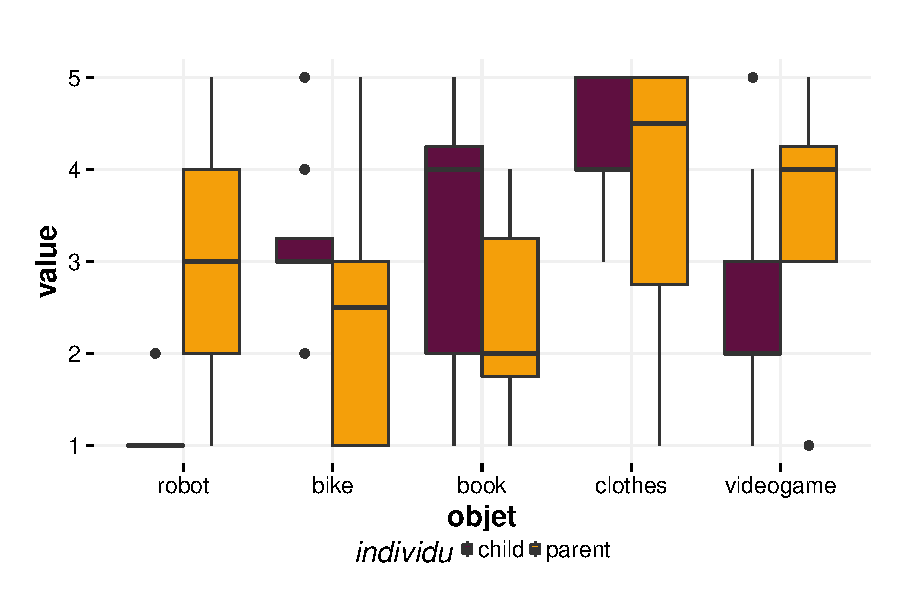
\includegraphics{interviews-plot_coirs_parent_enfant}

\subsubsection{Child-parent correlation in object ranking} 
Next graphs show the correlation between parent and children ranking for each of the child subject\newline
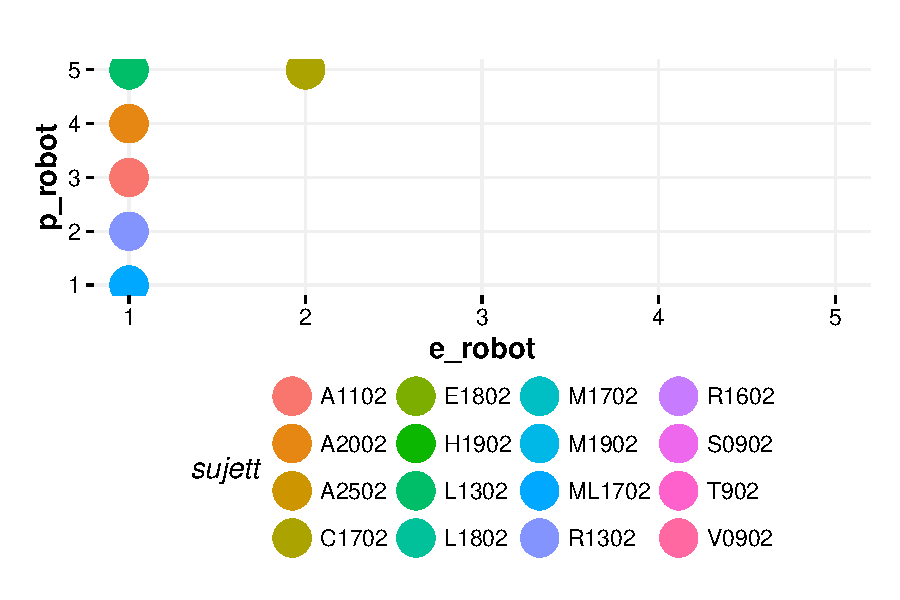
\includegraphics{interviews-plot_coirs_parent_enfant_robot}

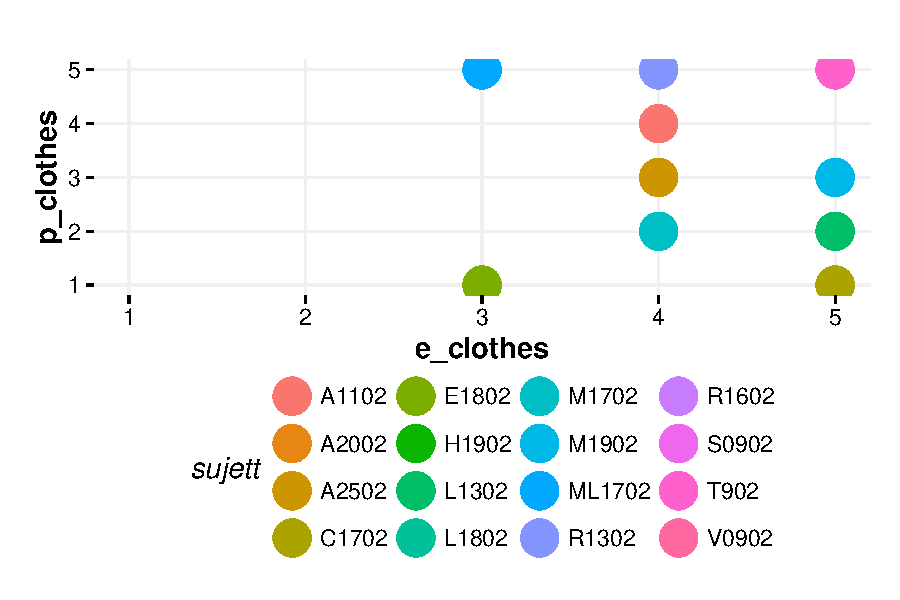
\includegraphics{interviews-plot_coirs_parent_enfant_clothes}

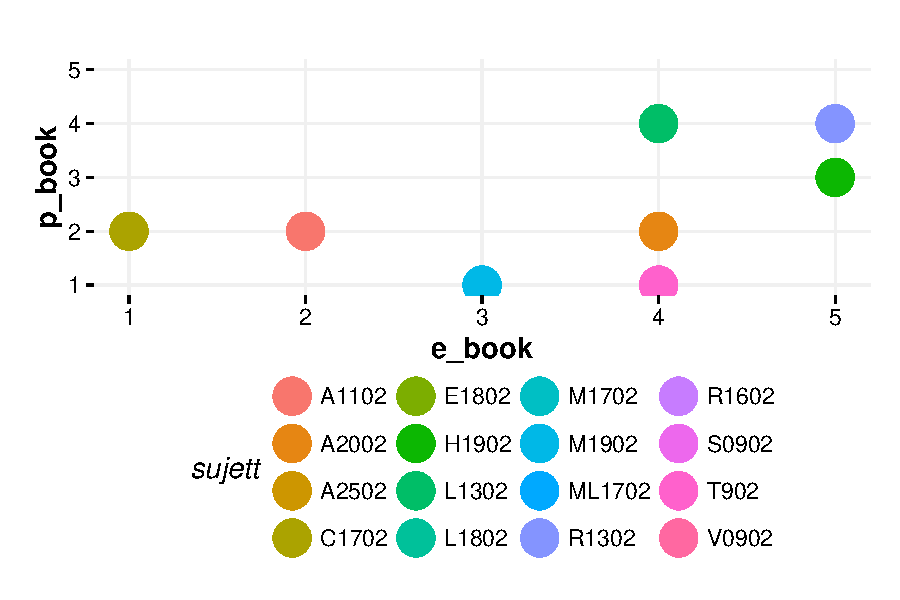
\includegraphics{interviews-plot_coirs_parent_enfant_book}

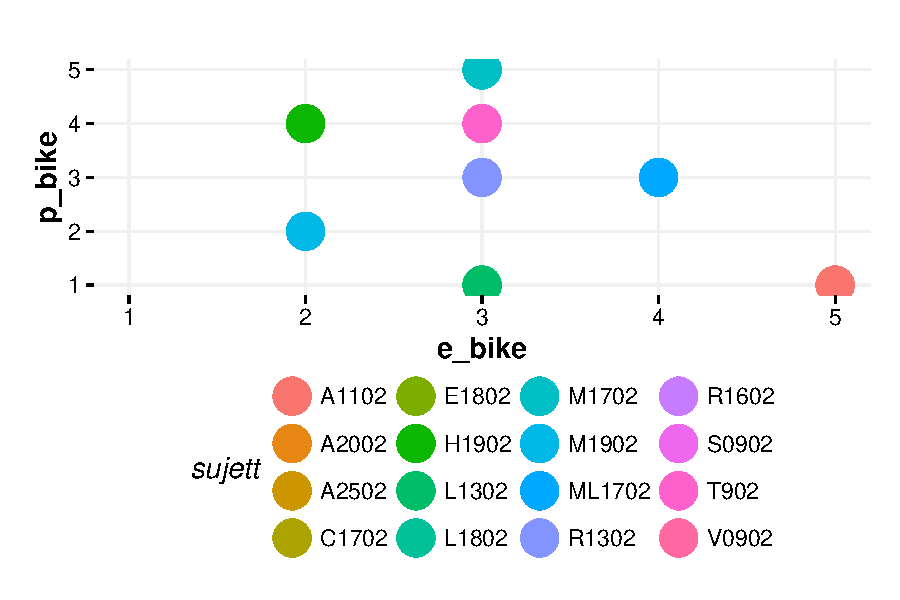
\includegraphics{interviews-plot_coirs_parent_enfant_bike}

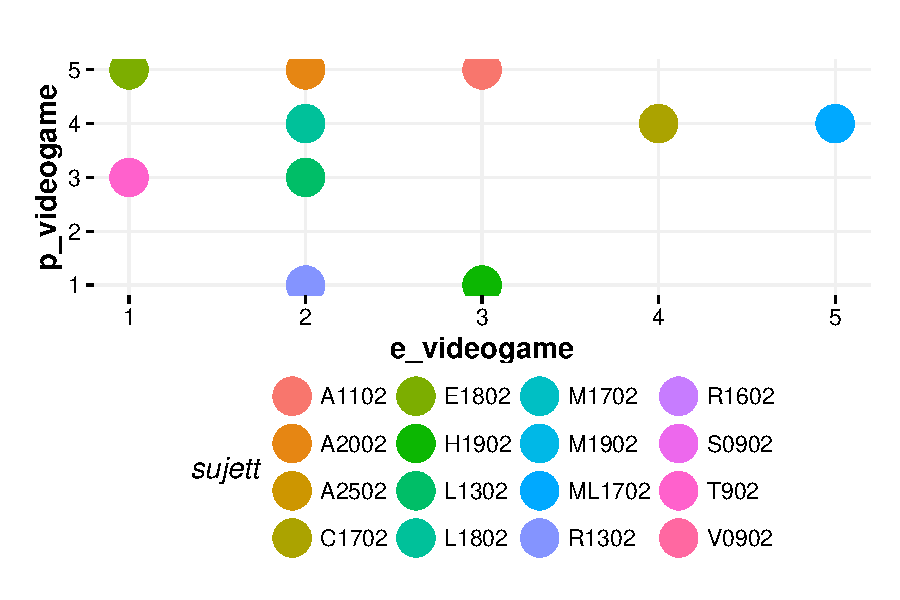
\includegraphics{interviews-plot_coirs_parent_enfant_videogame}

\subsection{Functionality preferences}

The following plot shows the average preference of children for each functionality (4: very preferred, 1: not preferred)

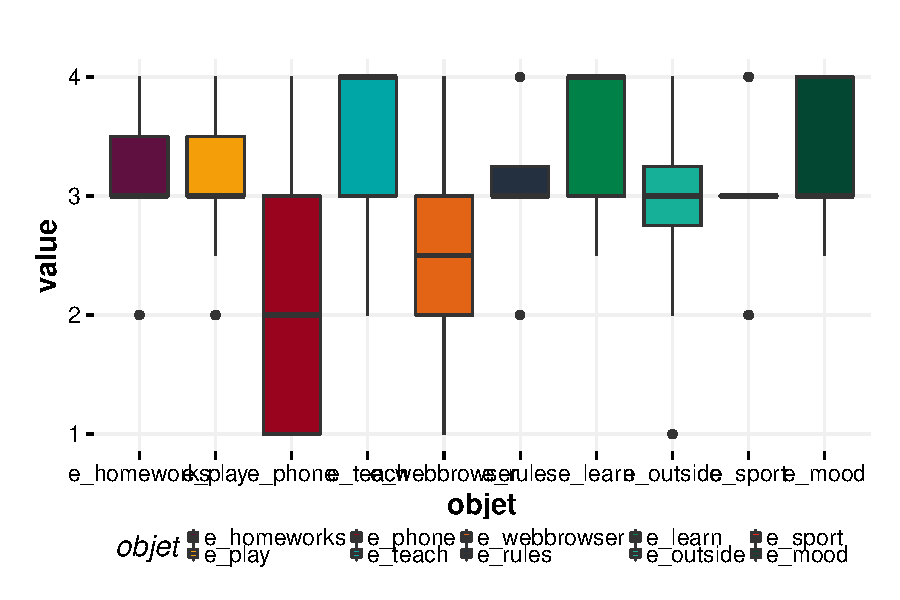
\includegraphics{interviews-plot_functionality_child}

The following plot shows the average preference of parents for each functionality (4: very preferred, 1: not preferred)
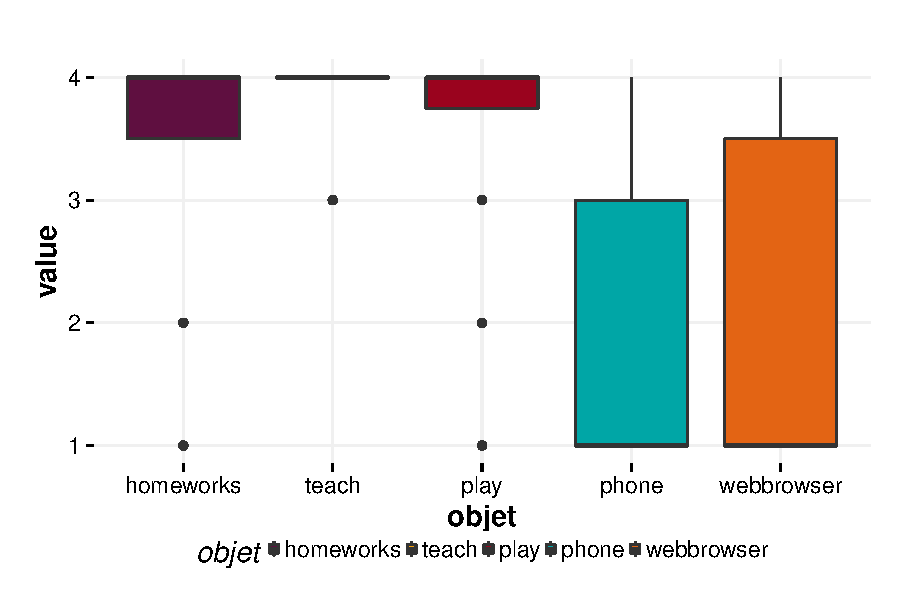
\includegraphics{interviews-plot_functionality_parent}

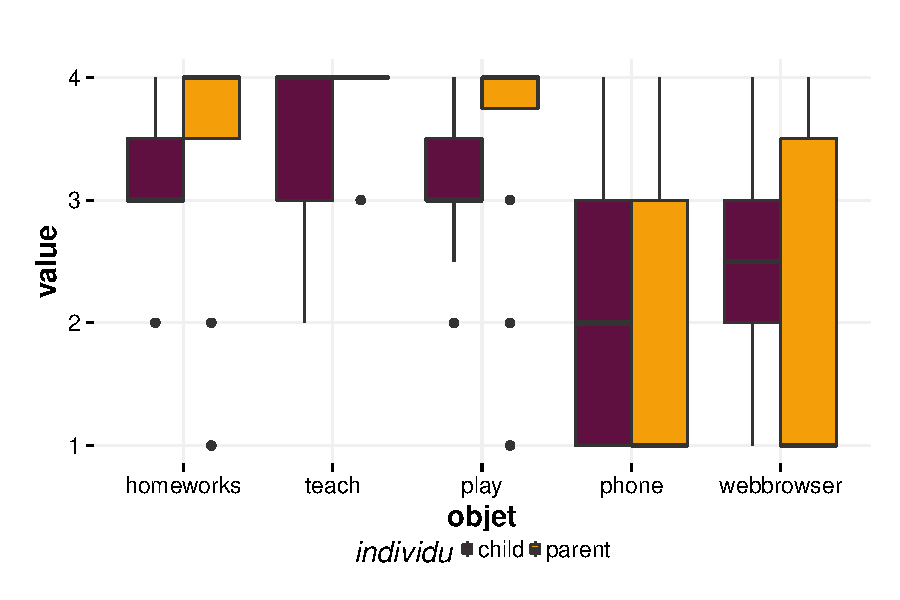
\includegraphics{interviews-plot_functionality_parent_enfant}




\section{Features}


\section{Postures}

\end{document}
